\PassOptionsToPackage{unicode=true}{hyperref} % options for packages loaded elsewhere
\PassOptionsToPackage{hyphens}{url}
%
\documentclass[]{article}
\usepackage{url}
\usepackage{graphicx} %use graph format
\usepackage{epstopdf}
\usepackage{lmodern}
\usepackage{amssymb,amsmath}
\usepackage{ifxetex,ifluatex}
\usepackage{fixltx2e} % provides \textsubscript
\ifnum 0\ifxetex 1\fi\ifluatex 1\fi=0 % if pdftex
  \usepackage[T1]{fontenc}
  \usepackage[utf8]{inputenc}
  \usepackage{textcomp} % provides euro and other symbols
\else % if luatex or xelatex
  \usepackage{unicode-math}
  \defaultfontfeatures{Ligatures=TeX,Scale=MatchLowercase}
\fi
% use upquote if available, for straight quotes in verbatim environments
\IfFileExists{upquote.sty}{\usepackage{upquote}}{}
% use microtype if available
\IfFileExists{microtype.sty}{%
\usepackage[]{microtype}
\UseMicrotypeSet[protrusion]{basicmath} % disable protrusion for tt fonts
}{}
\IfFileExists{parskip.sty}{%
\usepackage{parskip}
}{% else
\setlength{\parindent}{0pt}
\setlength{\parskip}{6pt plus 2pt minus 1pt}
}
\usepackage{hyperref}
\hypersetup{
            pdfborder={0 0 0},
            breaklinks=true}
\urlstyle{same}  % don't use monospace font for urls
\usepackage{color}
\usepackage{fancyvrb}
\newcommand{\VerbBar}{|}
\newcommand{\VERB}{\Verb[commandchars=\\\{\}]}
\DefineVerbatimEnvironment{Highlighting}{Verbatim}{commandchars=\\\{\}}
% Add ',fontsize=\small' for more characters per line
\newenvironment{Shaded}{}{}
\newcommand{\AlertTok}[1]{\textcolor[rgb]{1.00,0.00,0.00}{\textbf{#1}}}
\newcommand{\AnnotationTok}[1]{\textcolor[rgb]{0.38,0.63,0.69}{\textbf{\textit{#1}}}}
\newcommand{\AttributeTok}[1]{\textcolor[rgb]{0.49,0.56,0.16}{#1}}
\newcommand{\BaseNTok}[1]{\textcolor[rgb]{0.25,0.63,0.44}{#1}}
\newcommand{\BuiltInTok}[1]{#1}
\newcommand{\CharTok}[1]{\textcolor[rgb]{0.25,0.44,0.63}{#1}}
\newcommand{\CommentTok}[1]{\textcolor[rgb]{0.38,0.63,0.69}{\textit{#1}}}
\newcommand{\CommentVarTok}[1]{\textcolor[rgb]{0.38,0.63,0.69}{\textbf{\textit{#1}}}}
\newcommand{\ConstantTok}[1]{\textcolor[rgb]{0.53,0.00,0.00}{#1}}
\newcommand{\ControlFlowTok}[1]{\textcolor[rgb]{0.00,0.44,0.13}{\textbf{#1}}}
\newcommand{\DataTypeTok}[1]{\textcolor[rgb]{0.56,0.13,0.00}{#1}}
\newcommand{\DecValTok}[1]{\textcolor[rgb]{0.25,0.63,0.44}{#1}}
\newcommand{\DocumentationTok}[1]{\textcolor[rgb]{0.73,0.13,0.13}{\textit{#1}}}
\newcommand{\ErrorTok}[1]{\textcolor[rgb]{1.00,0.00,0.00}{\textbf{#1}}}
\newcommand{\ExtensionTok}[1]{#1}
\newcommand{\FloatTok}[1]{\textcolor[rgb]{0.25,0.63,0.44}{#1}}
\newcommand{\FunctionTok}[1]{\textcolor[rgb]{0.02,0.16,0.49}{#1}}
\newcommand{\ImportTok}[1]{#1}
\newcommand{\InformationTok}[1]{\textcolor[rgb]{0.38,0.63,0.69}{\textbf{\textit{#1}}}}
\newcommand{\KeywordTok}[1]{\textcolor[rgb]{0.00,0.44,0.13}{\textbf{#1}}}
\newcommand{\NormalTok}[1]{#1}
\newcommand{\OperatorTok}[1]{\textcolor[rgb]{0.40,0.40,0.40}{#1}}
\newcommand{\OtherTok}[1]{\textcolor[rgb]{0.00,0.44,0.13}{#1}}
\newcommand{\PreprocessorTok}[1]{\textcolor[rgb]{0.74,0.48,0.00}{#1}}
\newcommand{\RegionMarkerTok}[1]{#1}
\newcommand{\SpecialCharTok}[1]{\textcolor[rgb]{0.25,0.44,0.63}{#1}}
\newcommand{\SpecialStringTok}[1]{\textcolor[rgb]{0.73,0.40,0.53}{#1}}
\newcommand{\StringTok}[1]{\textcolor[rgb]{0.25,0.44,0.63}{#1}}
\newcommand{\VariableTok}[1]{\textcolor[rgb]{0.10,0.09,0.49}{#1}}
\newcommand{\VerbatimStringTok}[1]{\textcolor[rgb]{0.25,0.44,0.63}{#1}}
\newcommand{\WarningTok}[1]{\textcolor[rgb]{0.38,0.63,0.69}{\textbf{\textit{#1}}}}
\usepackage{graphicx,grffile}
\makeatletter
\def\maxwidth{\ifdim\Gin@nat@width>\linewidth\linewidth\else\Gin@nat@width\fi}
\def\maxheight{\ifdim\Gin@nat@height>\textheight\textheight\else\Gin@nat@height\fi}
\makeatother
% Scale images if necessary, so that they will not overflow the page
% margins by default, and it is still possible to overwrite the defaults
% using explicit options in \includegraphics[width, height, ...]{}
\setkeys{Gin}{width=\maxwidth,height=\maxheight,keepaspectratio}
\setlength{\emergencystretch}{3em}  % prevent overfull lines
\providecommand{\tightlist}{%
  \setlength{\itemsep}{0pt}\setlength{\parskip}{0pt}}
\setcounter{secnumdepth}{0}
% Redefines (sub)paragraphs to behave more like sections
\ifx\paragraph\undefined\else
\let\oldparagraph\paragraph
\renewcommand{\paragraph}[1]{\oldparagraph{#1}\mbox{}}
\fi
\ifx\subparagraph\undefined\else
\let\oldsubparagraph\subparagraph
\renewcommand{\subparagraph}[1]{\oldsubparagraph{#1}\mbox{}}
\fi

% set default figure placement to htbp
\makeatletter
\def\fps@figure{htbp}
\makeatother


\date{}

\begin{document}
\title{Simulation d'une loi gaussienne}
\author{Ruidong PAN \& Hengshuo LI}
\maketitle

\part*{Introduction}

Tous les langages de programmation possèdent un générateur de nombres
pseudo-aleatoires qui suit la loi uniforme sur l'interval $[0,1]$
. Le but de ce projet est de simuler une loi gaussienne en utilisant
deux variables aléatoires uniformes sur $[0,1]$ independantes pour
générer de nombres pseudo-aleatoires qui suit la loi $N(0;1)$.

\part*{Partie théorique }

Soient $U$ et $V$ deux variables aléatoires uniformes sur $[0,1]$
independantes:

\[
f_{U}(u)=\begin{cases}
1 & u\in\left[0,1\right]\\
0 & sinon
\end{cases}\qquad f_{V}(v)=\begin{cases}
1 & v\in\left[0,1\right]\\
0 & sinon
\end{cases}
\]

alors $X=\sqrt{-2log(u)}cos(2\pi V)$ et $Y=\sqrt{-2log(u)}sin(2\pi V)$
sont variables aléatoires indépendantes et de la loi $N(0;1)$.

\section*{Preuve}

Soient $X$ et $Y$ deux variables aléatoires indépendantes avec $X\sim N(0;1)$
et $Y\sim N(0;1)$, alors on a
\[
p(X,Y)\overbrace{=}^{ind\acute{e}pendantes}p(X)\times p(Y)=\frac{1}{\sqrt{2\pi}}e^{-\frac{X^{2}}{2}}\times\frac{1}{\sqrt{2\pi}}e^{-\frac{Y^{2}}{2}}=\frac{1}{2\pi}e^{-\frac{X^{2}+Y^{2}}{2}}
\]

En Transformant par coordonnées polaires avec $X=Rcos\theta$ et $Y=Rsin\theta$
où $\theta\in[0,2\pi]$, on obtient :

\[
\frac{1}{2\pi}e^{-\frac{X^{2}+Y^{2}}{2}}=\frac{1}{2\pi}e^{-\frac{R^{2}}{2}}
\]

Or on sait que : $\iint_{D}f(x,y)dxdy=\int_{\beta}^{\alpha}d\theta\int_{\rho_{1}(\theta)}^{\rho_{2}(\theta)}f(\rho cos\theta,\rho sin\theta)\rho d\rho$

Alors on a :

\[
\int_{-\infty}^{\infty}\int_{-\infty}^{\infty}\frac{1}{2\pi}e^{-\frac{X^{2}+Y^{2}}{2}}dXdY=\int_{-\infty}^{\infty}\int_{-\infty}^{\infty}\frac{1}{2\pi}e^{-\frac{R^{2}}{2}}Rd\theta dR=1
\]

On a donc aussi la fonction de répartition pour $R$ et $\theta$
:

\[
F_{R}(R\leqslant r)=\int_{0}^{r}\int_{0}^{2\pi}\frac{1}{2\pi}e^{-\frac{R^{2}}{2}}Rd\theta dR
\]

\[
\qquad\quad\quad=\int_{0}^{r}\left(\int_{0}^{2\pi}\frac{1}{2\pi}Re^{-\frac{R^{2}}{2}}d\theta\right)dR
\]

\[
=\int_{0}^{r}Re^{-\frac{R^{2}}{2}}dR
\]

\[
\qquad\quad=-\left[e^{-\frac{R^{2}}{2}}\right]_{0}^{r}=1-e^{-\frac{r^{2}}{2}}
\]

\[
F_{\theta}(\theta\leqslant\phi)=\int_{0}^{\phi}\int_{0}^{\infty}\frac{1}{2\pi}e^{-\frac{R^{2}}{2}}Rd\theta dR
\]

\[
=\int_{0}^{\phi}\left(\int_{0}^{\infty}\frac{1}{2\pi}Re^{-\frac{R^{2}}{2}}dR\right)d\theta
\]

\[
=\int_{0}^{\phi}\frac{1}{2\pi}\left[-e^{-\frac{R^{2}}{2}}\right]_{0}^{\infty}d\theta
\]

\[
=\int_{0}^{\phi}\frac{1}{2\pi}d\theta=\frac{\phi}{2\pi}
\]

Soient $U_{1}$ et $U_{2}$ deux variables aléatoires independantes
uniformes sur $[0,1]$, on peut prendre $\theta=2\pi U_{2}$, car
$F_{\theta}(\theta\leqslant\phi)=\frac{\phi}{2\pi}$, $\theta$ est
uniformes sur $[0,2\pi]$.

$F_{R}(R\leqslant r)=1-e^{-\frac{r^{2}}{2}}$ donc on peut obtenir
$R=F_{R}^{-1}(z)=\sqrt{-2ln(1-z)}$, d'après la méthode de la transformée
inverse, la variable aléatoire $R=F_{R}^{-1}(z)$ a pour fonction
de répartition $F_{R}(R\leqslant r)$, où $z$ est une variable aléatoire
de loi uniforme sur $[0;1]$. Or si $z$ est uniforme, alors $(1-z)$
est aussi uniforme. Pour notre cas, $z$ est uniforme sur $[0,1]$,
donc $(1-z)$ est aussi uniforme sur $[0,1]$. Et on peut prendre
$U_{1}=(1-z)$.

Enfin, on peut obtenir $X=Rcos\theta=\sqrt{-2lnU_{1}}cos(2\pi U_{2})$
et $Y=Rsin\theta=\sqrt{-2lnU_{1}}sin(2\pi U_{2})$ où $X$ et $Y$
sont deux variables aléatoires indépendantes de la loi $N(0;1)$.

Donc on peut conclure que on n'a besoin que de deux variables aléatoires
independantes $U_{1}$ et $U_{2}$ qui suivent la loi uniforme sur
$[0,1]$, alors on peut obtenir une variable aléatoire de la loi $N(0;1)$
soit par la formule $\sqrt{-2lnU_{1}}cos(2\pi U_{2})$ soit par $\sqrt{-2lnU_{1}}sin(2\pi U_{2})$.
Cette conclusion s'appelle aussi la méthode de la transformation de
Box-Muller.

CQFD.

\part*{Partie appliquée avec le code}

\hypertarget{header-n501}{%
\subsection{Mise en oeuvre informatique }\label{header-n501}}

Nous utilisons langage C pour réaliser la programme.

\hypertarget{header-n504}{%
\paragraph{Code pour créer les données entre 0 et 1}\label{header-n504}}

\begin{Shaded}
\begin{Highlighting}[]
\DataTypeTok{float}\NormalTok{ rm()\{}
     \DataTypeTok{float}\NormalTok{ c= rand()/(}\DataTypeTok{double}\NormalTok{)(RAND_MAX + }\FloatTok{1.0}\NormalTok{);}
     \ControlFlowTok{return}\NormalTok{ c;}
\NormalTok{\}}
\end{Highlighting}
\end{Shaded}

\hypertarget{header-n506}{%
\paragraph{Code permettant d'obtenir les données pour simuler une
gaussienne }\label{header-n506}}

\begin{Shaded}
\begin{Highlighting}[]
\DataTypeTok{void}\NormalTok{ gaussienne(}\DataTypeTok{float}\NormalTok{ U[max] ,}\DataTypeTok{float}\NormalTok{ V[max],}\DataTypeTok{float}\NormalTok{ m,}\DataTypeTok{float}\NormalTok{ n,}\DataTypeTok{float}\NormalTok{ t,coord C[max])\{}
\NormalTok{       n=sqrt(n);}
       \DataTypeTok{float}\NormalTok{ tmp1, tmp2;}
       \ControlFlowTok{for}\NormalTok{ (}\DataTypeTok{int}\NormalTok{ j=}\DecValTok{0}\NormalTok{; j< t; j++)\{}
\NormalTok{                tmp1 = -}\DecValTok{2}\NormalTok{*log(U[j]);}
\NormalTok{                tmp2 = }\DecValTok{2}\NormalTok{*PI*V[j];}
\NormalTok{                C[j].x=m+n* sqrt(tmp1)*sin(tmp2);}
\NormalTok{                C[j].y=m+n* sqrt(tmp1)*cos(tmp2);     \}}

\NormalTok{\}}
\end{Highlighting}
\end{Shaded}

Ensuite nous traitons les données pour calculer sa fréquence et faire
des histogrammes

\hypertarget{header-n509}{%
\paragraph{Code permettant d'obtenir histogramme de données de
gaussienne }\label{header-n509}}

\begin{Shaded}
\begin{Highlighting}[]
\DataTypeTok{void}\NormalTok{ hist1(}\DataTypeTok{int}\NormalTok{ t ,}\DataTypeTok{int}\NormalTok{ nb,}\DataTypeTok{float}\NormalTok{ m,}\DataTypeTok{float}\NormalTok{ n,coord C[max] )\{}
       \DataTypeTok{float}\NormalTok{ xb[N]; }\DataTypeTok{int}\NormalTok{ a[N];}
       \DataTypeTok{float}\NormalTok{ da;}
\NormalTok{       da = }\FloatTok{2.0}\NormalTok{ * SCOPE * sqrt(n) / nb;}
       \ControlFlowTok{for}\NormalTok{ (}\DataTypeTok{int}\NormalTok{ i=}\DecValTok{0}\NormalTok{; i<=nb;i++) \{}
\NormalTok{               xb[i]=m-SCOPE * sqrt((}\DataTypeTok{double}\NormalTok{)n)+ i * da;}
\NormalTok{       \}}
       \ControlFlowTok{for}\NormalTok{ (}\DataTypeTok{int}\NormalTok{ i=}\DecValTok{0}\NormalTok{; i<nb; i++) a[i]=}\DecValTok{0}\NormalTok{;}
       \ControlFlowTok{for}\NormalTok{ (}\DataTypeTok{int}\NormalTok{ i =}\DecValTok{0}\NormalTok{; i< t;i++ )\{}
               \ControlFlowTok{for}\NormalTok{ (}\DataTypeTok{int}\NormalTok{ j=}\DecValTok{0}\NormalTok{;j<nb; j++)\{}
               \ControlFlowTok{if}\NormalTok{ (contain(C[i].x,xb[j],xb[j+}\DecValTok{1}\NormalTok{])==}\DecValTok{1}\NormalTok{) \{}
\NormalTok{               a[j]+=}\DecValTok{1}\NormalTok{;}
               \ControlFlowTok{break}\NormalTok{;}
\NormalTok{               \}}
\NormalTok{               \}}

\NormalTok{       \}}
       \DataTypeTok{float}\NormalTok{ mean, proba;}
       \ControlFlowTok{for}\NormalTok{(}\DataTypeTok{int}\NormalTok{ i=}\DecValTok{0}\NormalTok{ ; i<nb;i++)\{}
\NormalTok{               mean=}\FloatTok{0.5}\NormalTok{* ( xb[i] + xb[i+}\DecValTok{1}\NormalTok{]);}
\NormalTok{               proba=a[i]/(da*t);}
\NormalTok{               printf(}\StringTok{" %f %f}\SpecialCharTok{\textbackslash{}n}\StringTok{"}\NormalTok{,mean,proba);}
\NormalTok{       \}}

\NormalTok{\}}
\end{Highlighting}
\end{Shaded}

\hypertarget{header-n511}{%
\paragraph{Code pour histogramme des données aléatoires fabriqué par
générateur de nombre aléatoires}\label{header-n511}}

\begin{Shaded}
\begin{Highlighting}[]
\DataTypeTok{void}\NormalTok{ hist2(}\DataTypeTok{int}\NormalTok{ t ,}\DataTypeTok{int}\NormalTok{ nb , }\DataTypeTok{float}\NormalTok{ U[max] )\{}
       \DataTypeTok{float}\NormalTok{ xbb[N] ;  }\DataTypeTok{int}\NormalTok{ aa[N] ;}
       \DataTypeTok{float}\NormalTok{ da = }\FloatTok{1.0}\NormalTok{ / nb;}
       \ControlFlowTok{for}\NormalTok{ (}\DataTypeTok{int}\NormalTok{ i=}\DecValTok{0}\NormalTok{;  i<=nb;i++)  xbb[i] = i*da;}
       \ControlFlowTok{for}\NormalTok{ (}\DataTypeTok{int}\NormalTok{ i=}\DecValTok{0}\NormalTok{; i<nb; i++) aa[i]=}\DecValTok{0}\NormalTok{;}

       \ControlFlowTok{for}\NormalTok{ (}\DataTypeTok{int}\NormalTok{ i =}\DecValTok{0}\NormalTok{; i< t;i++ )\{}

               \ControlFlowTok{for}\NormalTok{ (}\DataTypeTok{int}\NormalTok{ j=}\DecValTok{0}\NormalTok{;j<nb;j ++)\{}
                       \ControlFlowTok{if}\NormalTok{ (contain(U[i],xbb[j],xbb[j+}\DecValTok{1}\NormalTok{])== }\DecValTok{0}\NormalTok{) }\ControlFlowTok{continue}\NormalTok{;}
\NormalTok{                       aa[j]+=}\DecValTok{1}\NormalTok{;}
                       \ControlFlowTok{break}\NormalTok{;}

\NormalTok{               \}}
\NormalTok{       \}}

       \DataTypeTok{float}\NormalTok{ mean, proba;}
       \ControlFlowTok{for}\NormalTok{(}\DataTypeTok{int}\NormalTok{ i=}\DecValTok{0}\NormalTok{ ; i<nb;i++)\{}
\NormalTok{               mean=}\FloatTok{0.5}\NormalTok{* (xbb[i] + xbb[i+}\DecValTok{1}\NormalTok{]);}
\NormalTok{               proba=aa[i]/(t*da);}
\NormalTok{               printf(}\StringTok{" %f %f}\SpecialCharTok{\textbackslash{}n}\StringTok{"}\NormalTok{, mean,proba);}
\NormalTok{       \}}



\NormalTok{\}}
\end{Highlighting}
\end{Shaded}

\hypertarget{header-n513}{%
\paragraph{Code pour histogramme des doneées gausienne en dimension deux
pour vérifier indépendances}\label{header-n513}}

\begin{Shaded}
\begin{Highlighting}[]
\DataTypeTok{void}\NormalTok{ hist3(}\DataTypeTok{int}\NormalTok{ t ,}\DataTypeTok{int}\NormalTok{ nb,}\DataTypeTok{float}\NormalTok{ m,}\DataTypeTok{float}\NormalTok{ n,coord C[max]  )\{}
\NormalTok{       coord xc[N][N]; }\DataTypeTok{int}\NormalTok{ ac[N][N];}
       \DataTypeTok{float}\NormalTok{ da  =}\DecValTok{2}\NormalTok{ * SCOPE * sqrt((}\DataTypeTok{double}\NormalTok{)n)/nb;}
       \ControlFlowTok{for}\NormalTok{ (}\DataTypeTok{int}\NormalTok{ i=}\DecValTok{0}\NormalTok{; i<=nb; i++) \{}
              \ControlFlowTok{for}\NormalTok{ (}\DataTypeTok{int}\NormalTok{ j=}\DecValTok{0}\NormalTok{;j<=nb;j++)\{}
\NormalTok{                      xc[i][j].x=m-SCOPE * sqrt(n)+i*da;}
\NormalTok{                      xc[i][j].y=m-SCOPE * sqrt(n)+j*da;}
\NormalTok{              \}}
\NormalTok{       \}}
       \ControlFlowTok{for}\NormalTok{ (}\DataTypeTok{int}\NormalTok{ i=}\DecValTok{0}\NormalTok{ ; i<nb ; i++)}
               \ControlFlowTok{for}\NormalTok{ (}\DataTypeTok{int}\NormalTok{ j =}\DecValTok{0}\NormalTok{; j< nb ; j++)}
\NormalTok{                       ac[i][j]=}\DecValTok{0}\NormalTok{;}

       \ControlFlowTok{for}\NormalTok{ (}\DataTypeTok{int}\NormalTok{ i =}\DecValTok{0}\NormalTok{; i< t ;i++ )\{}
               \ControlFlowTok{for}\NormalTok{ (}\DataTypeTok{int}\NormalTok{ j=}\DecValTok{0}\NormalTok{;j<nb; j++)\{}
                       \ControlFlowTok{if}\NormalTok{ (contain(C[i].x,xc[j][}\DecValTok{0}\NormalTok{].x,xc[j+}\DecValTok{1}\NormalTok{][}\DecValTok{0}\NormalTok{].x)==}\DecValTok{1}\NormalTok{)\{}
                          \ControlFlowTok{for}\NormalTok{ (}\DataTypeTok{int}\NormalTok{ k=}\DecValTok{0}\NormalTok{; k<nb; k++)\{}
                              \ControlFlowTok{if}\NormalTok{ (contain(C[i].y , xc[j][k].y , xc[j][k+}\DecValTok{1}\NormalTok{].y)==}\DecValTok{1}\NormalTok{) \{}
\NormalTok{                                      ac[j][k]+=}\DecValTok{1}\NormalTok{;}
                                      \ControlFlowTok{break}\NormalTok{;}
\NormalTok{                              \}}
\NormalTok{                          \}}
                          \ControlFlowTok{break}\NormalTok{;}
\NormalTok{                       \}}

\NormalTok{               \}}
\NormalTok{       \}}

       \DataTypeTok{float}\NormalTok{ meanx,meany,proba;}

       \ControlFlowTok{for}\NormalTok{(}\DataTypeTok{int}\NormalTok{ i=}\DecValTok{0}\NormalTok{ ; i<nb;i++ )\{}
               \ControlFlowTok{for}\NormalTok{ (}\DataTypeTok{int}\NormalTok{ j=}\DecValTok{0}\NormalTok{;j<nb;j++)\{}
\NormalTok{                      meanx=}\FloatTok{0.5}\NormalTok{*(xc[i][j].x + xc[i+}\DecValTok{1}\NormalTok{][j].x);}
\NormalTok{                      meany=}\FloatTok{0.5}\NormalTok{*(xc[i][j].y+xc[i][j+}\DecValTok{1}\NormalTok{].y);}
\NormalTok{                      proba=ac[i][j]/(da*da*t);}
\NormalTok{                      printf(}\StringTok{" %f %f %f}\SpecialCharTok{\textbackslash{}n}\StringTok{"}\NormalTok{, meanx, meany, proba);\}}
\NormalTok{               \}}
\NormalTok{\}}
\end{Highlighting}
\end{Shaded}

\hypertarget{header-n515}{%
\paragraph{Code de main program}\label{header-n515}}

\begin{Shaded}
\begin{Highlighting}[]
\DataTypeTok{int}\NormalTok{ main()}
\NormalTok{\{       srand(time(NULL));}
        \DataTypeTok{float}\NormalTok{ U[max],V[max],X[max]; coord C[max];}
        \DataTypeTok{float}\NormalTok{ m,n;}
        \DataTypeTok{int}\NormalTok{ t,nb;}
        \DataTypeTok{int}\NormalTok{ cho;}
\NormalTok{        scanf(}\StringTok{"%f %f %d %d %d"}\NormalTok{,&m,&n,&t,&nb,&cho);}
        \ControlFlowTok{for}\NormalTok{ (}\DataTypeTok{int}\NormalTok{ i=}\DecValTok{0}\NormalTok{; i < t; i++)\{}
\NormalTok{        U[i]=rm();}
\NormalTok{        V[i]=rm();\}}
\NormalTok{        gaussienne(U,V,m,n,t,C);}
        \ControlFlowTok{switch}\NormalTok{(cho)\{}
                \ControlFlowTok{case} \DecValTok{1}\NormalTok{ :}
\NormalTok{                hist1(t,nb,m,n,C);}
                \ControlFlowTok{break}\NormalTok{;}
                \ControlFlowTok{case} \DecValTok{2}\NormalTok{ :}
\NormalTok{                hist2(t,nb,U);}
                \ControlFlowTok{break}\NormalTok{;}
                \ControlFlowTok{case} \DecValTok{3}\NormalTok{ :}
\NormalTok{                hist3(t,nb,m,n,C);}
                \ControlFlowTok{break}\NormalTok{;}
\NormalTok{        \}}
        \ControlFlowTok{return} \DecValTok{0}\NormalTok{;}
\NormalTok{\}}
\end{Highlighting}
\end{Shaded}

\hypertarget{header-n517}{%
\subsection{L'analyse des données}\label{header-n517}}

\hypertarget{header-n518}{%
\paragraph{Loi de uniforme }\label{header-n518}}

Nous pouvons utiliser le fonction \texttt{srand()} et \texttt{rand()}
pour obtenir des données entre (0,1). Et nous les transformons en images
de fonction densité de probabilité et comparons avec la loi de
uniforme.\\
\begin{figure}
	\centering
	\includegraphics[height=6cm,width=11cm]{images/U01.png}
	\caption{la fonction de densité de loi de uniforme U(0,1)}
	\label{fig1}
\end{figure}

\begin{figure}
	\centering
	\includegraphics[height=6cm,width=11cm]{images/iU01.png}
	\caption{les données nous simulons loi de uniforme}
	\label{fig2}
\end{figure}

Ce sont les données nous en prenons cent mille. Elles ne peuvent pas
strictement obéir à la distribution uniforme et elles fluctuent entre
(-0.1,0.1). Peut-être le méthode que nous utilisons n'est pas si
aléatoire, mais ca ira.

\hypertarget{header-n521}{%
\paragraph{Loi de normale (méthode de gaussienne)}\label{header-n521}}

La but de ce projet est que on simule les variables aléatoire gaussienne
et on traite les données pour faites en une image de distributions
probabilitées pour vérifier s'il s'agit d'un le loi de normale. \\
\begin{figure}
	\centering
	\includegraphics[height=6cm,width=11cm]{images/N01.png}
	\caption{la loi de normale}
	\label{fig3}
\end{figure}
\begin{figure}
	\centering
	\includegraphics[height=6cm,width=11cm]{images/iN01.png}
	\caption{les données nous simulons avec les variable gaussienne}
	\label{fig4}
\end{figure}

Nous constatons des deux images sont cohérent. Donc ca nous permet de
dire la simulation de gaussienne est bien réussite. Simultanément, on
simuler les variable aléatoire gaussienne avec moyenne et
varience(comparer avec la fonction de densitées de loi normale avec le
même moyenne et varience), ce sont des images.\\

\begin{figure}
	\centering
	\includegraphics[height=6cm,width=11cm]{images/iN302.png}
	\caption{iN(3,0.2)}
	\label{fig5}
\end{figure}

\begin{figure}
	\centering
	\includegraphics[height=6cm,width=11cm]{images/N302.png}
	\caption{N(3,0.2)}
	\label{fig6}
\end{figure}

\begin{figure}
	\centering
	\includegraphics[height=6cm,width=11cm]{images/iN306.png}
	\caption{iN(3,0.6)}
	\label{fig7}
\end{figure}

\begin{figure}
	\centering
	\includegraphics[height=6cm,width=11cm]{images/N306.png}
	\caption{N(3,0.6) }
	\label{fig8}
\end{figure}

\begin{figure}
	\centering
	\includegraphics[height=6cm,width=11cm]{images/iN-510.png}
	\caption{iN(-5,10)}
	\label{fig9}
\end{figure}

\begin{figure}
	\centering
	\includegraphics[height=6cm,width=11cm]{images/N-510.png}
	\caption{N(-5,10)}
	\label{fig10}
\end{figure}

\begin{figure}
	\centering
	\includegraphics[height=6cm,width=11cm]{images/iN-520.png}
	\caption{iN(-5,20)}
	\label{fig11}
\end{figure}

\begin{figure}
	\centering
	\includegraphics[height=6cm,width=11cm]{images/N-520.png}
	\caption{N(-5,20)}
	\label{fig12}
\end{figure}
Bien que leurs formes soient similaires, mais leurs échelles d'abscisses
sont différentes. C'est dommage que je ne puisse pas les mettre dans une
seule image.

\hypertarget{header-n524}{%
\paragraph{La loi de normale en dimension 2(méthode de
gausienne)}\label{header-n524}}

On veut vérifier des deux varaibles \(X\) et \(Y\) s'il sont
indépendant. Pendant ce temps on veut aussi vérifier la démonstration qu'on fait
avant. La variable \(X\) est dans un dimension et \(Y\) est dans l'autre
dimension, on vois que s'il peut fabriquer la fonction de densités dans
dimension deux. voici les résultat:\\

\begin{figure}
	\centering
	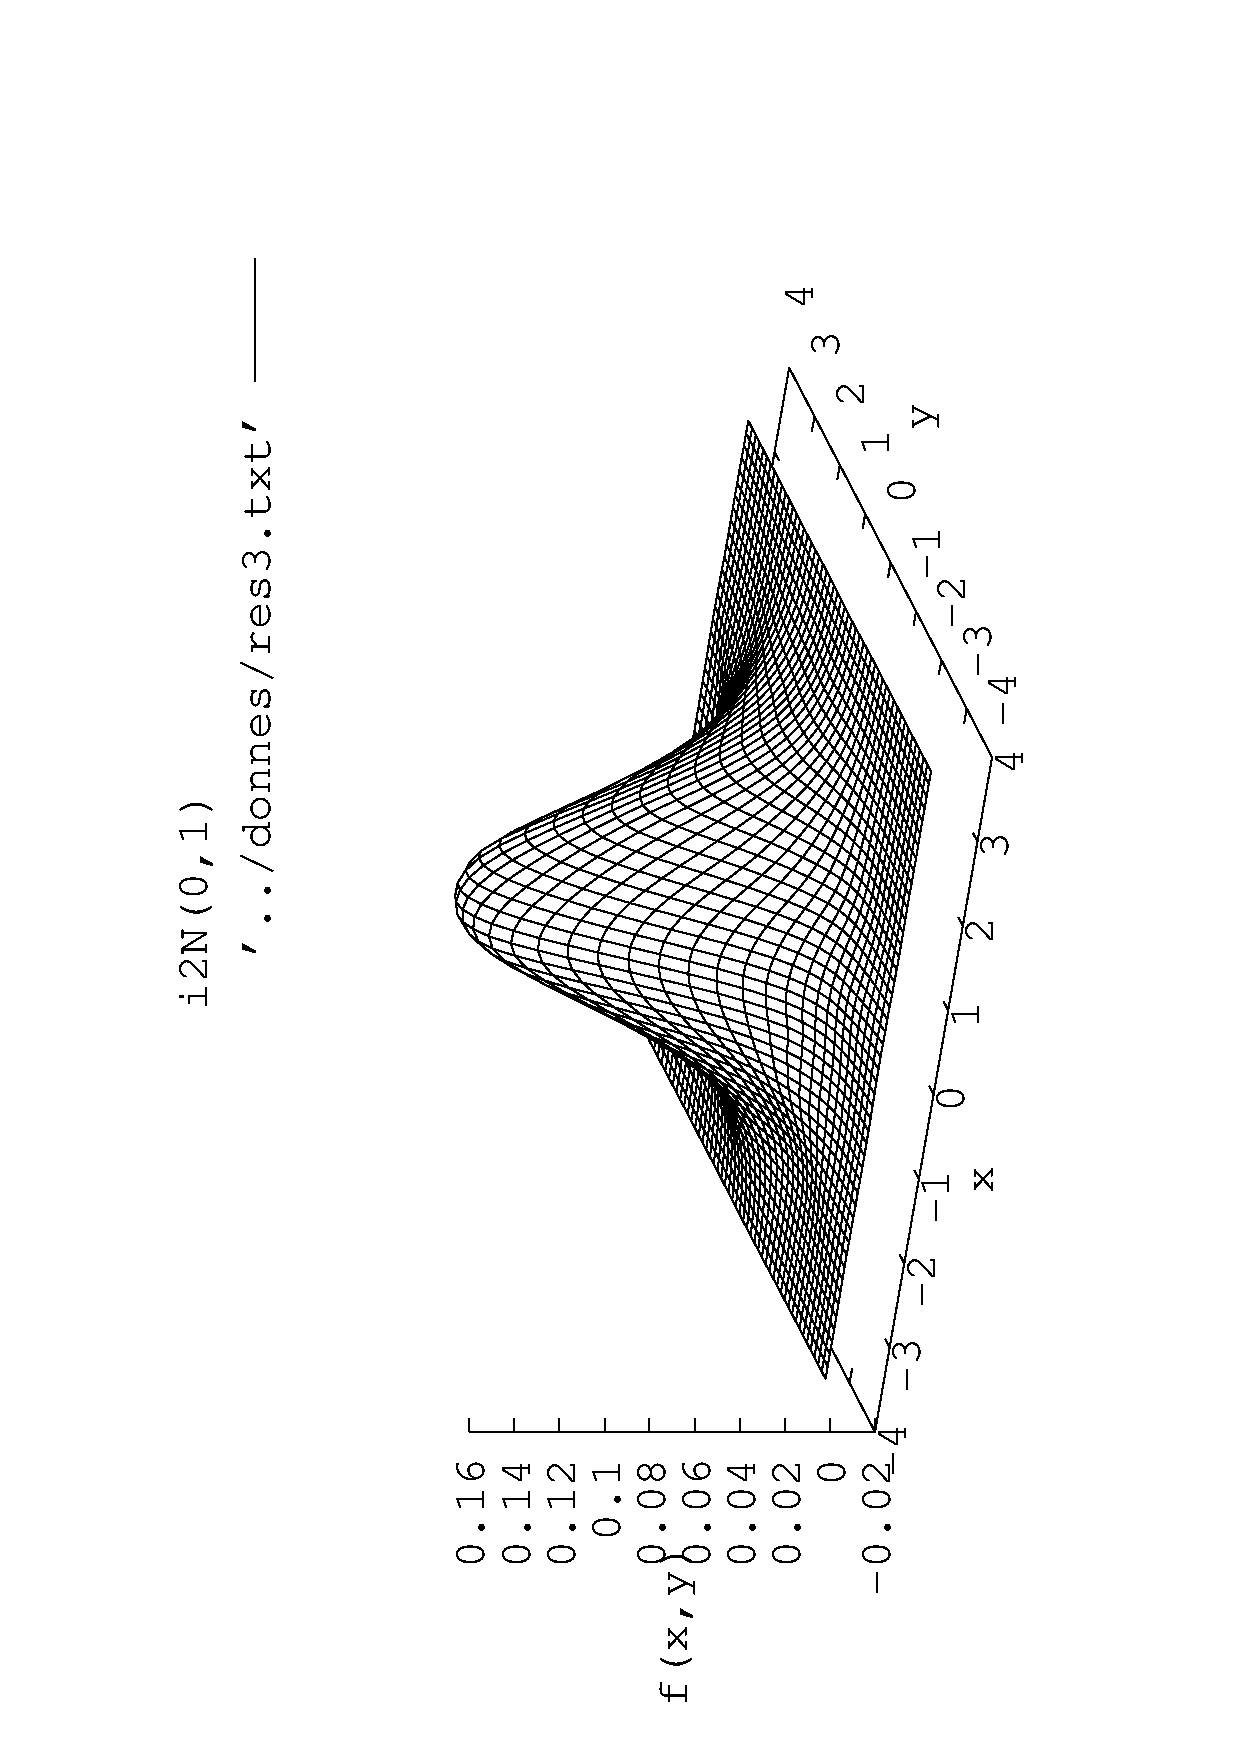
\includegraphics[height=6cm,width=11cm]{images/2iN01.png}
	\caption{2iN(0,1)}
	\label{fig13}
\end{figure}
Elle est bien symétrique, uniforme. on la compare avec le fonction de
densité de loi de normale en deux dimension:\\

\begin{figure}
	\centering
	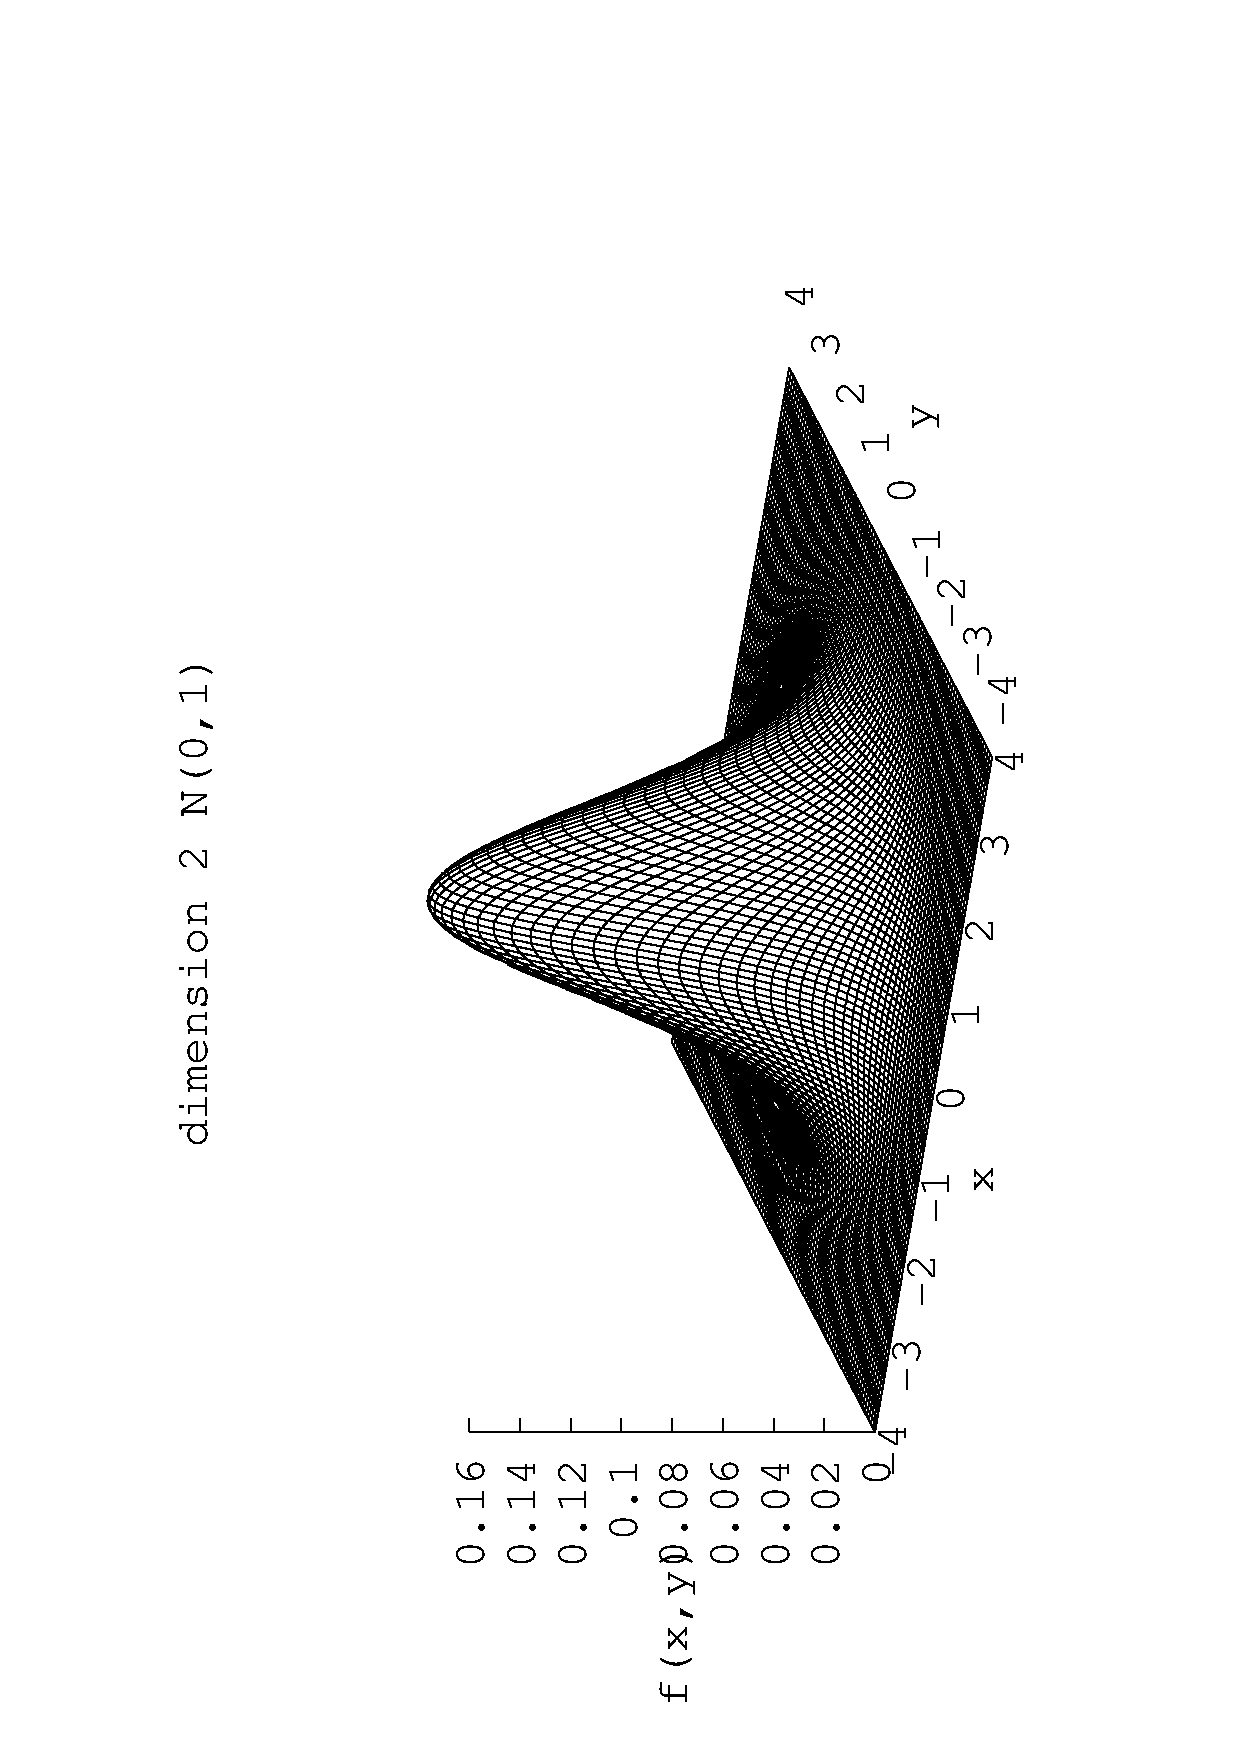
\includegraphics[height=6cm,width=11cm]{images/2N01.png}
	\caption{2N(0,1)}
	\label{fig14}
\end{figure}
Nous constatons ce sont identique. Donc on peut dire que la
démonstration a la raisons et \(X\) et \(Y\) sont bien ondépendant.

\hypertarget{header-n526}{%
\part*{Conclusion}\label{header-n526}}

Nous mettons les projet en oeuvre en 3 partie. D'aborde on démonstre la
méthode gaussienne comment il se connect avec la loi de uniforme. Et
puis nous programmeons la code et nous débuggeons. Au final, nous
traitons des données en images. \\
Nous avons compris comment utiliser les générateur de nombres aléatoire
pour obtient les varaibles gausiennes. la précision dépende du caractère
aléatoire des nombre générée par générateur. C'est une méthode très
pratique, simple et pas beaucoup de calcul pour PC. \\
Nous avons compris comment utiliser gnuplot pour faire des images avec des
données.\\
Nous constatons les limite mémoire quand on teste les data, pour mon
ordinateur il peut pas traiter au plus de un million de deux integer(8
octets) pour tableaux.

\hypertarget{header-n528}{%
	\begin{thebibliography}{99}\label{header-n528}}

		\bibitem{crs01} RO-projet2.pdf \\
		\bibitem{crs02} \url{http://fr.wikipedia.org/wiki/Méthode_de_Box-Muller}
	\end{thebibliography}

\end{document}
